% Source: Code/xband-radar-sim/docs/radar_simulation_technical.tex
% Description: Echo timing. The echo arrives after round-trip delay $\tau = 2R/c$ with amplitude $A$ and phase $\phi$.

\documentclass[border=4pt]{standalone}
\usepackage{algpseudocode}
\usepackage{amsmath,amssymb,amsfonts}
\usepackage[T1]{fontenc}
\usepackage{graphicx}
\usepackage{pgfplots}
\usepackage{tikz}
\usepackage{xcolor}
\pgfplotsset{compat=1.18}
\usetikzlibrary{arrows.meta,positioning,shapes.geometric,calc,patterns,decorations.pathmorphing,3d,angles,quotes}

\definecolor{radargreen}{RGB}{0,255,0}
\definecolor{raycolor}{RGB}{255,165,0}
\definecolor{targetcolor}{RGB}{255,0,0}
\definecolor{groundcolor}{RGB}{139,90,43}
\definecolor{skycolor}{RGB}{135,206,235}
\definecolor{beamcolor}{RGB}{255,255,0}


\begin{document}
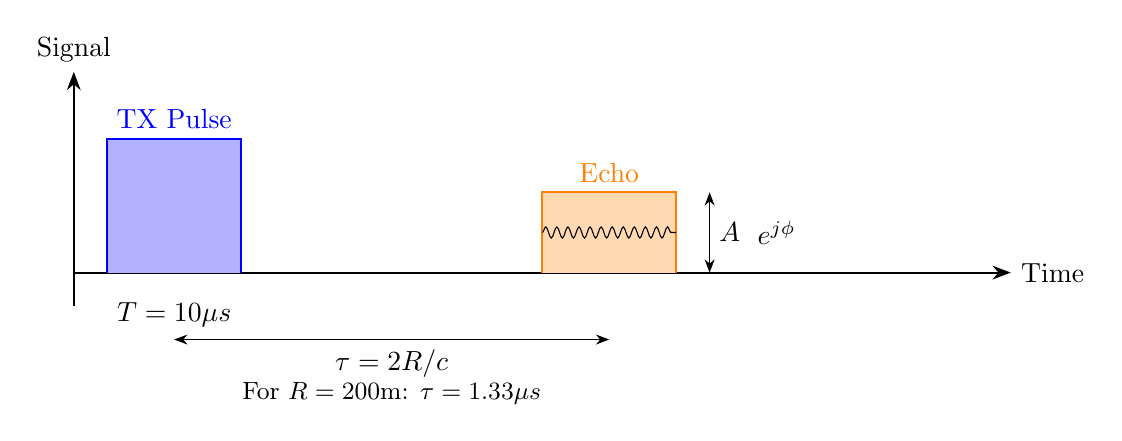
\begin{tikzpicture}[scale=0.85]
    % Timeline
    \draw[-{Stealth}, thick] (0,0) -- (14,0) node[right] {Time};
    \draw[-{Stealth}, thick] (0,-0.5) -- (0,3) node[above] {Signal};

    % TX pulse
    \fill[blue!30] (0.5,0) rectangle (2.5,2);
    \draw[thick, blue] (0.5,0) -- (0.5,2) -- (2.5,2) -- (2.5,0);
    \node[blue, above] at (1.5,2) {TX Pulse};
    \node[below] at (1.5,-0.3) {$T = 10\mu s$};

    % Echo (delayed)
    \fill[orange!30] (7,0) rectangle (9,1.2);
    \draw[thick, orange] (7,0) -- (7,1.2) -- (9,1.2) -- (9,0);
    \node[orange, above] at (8,1.2) {Echo};

    % Delay annotation
    \draw[{Stealth}-{Stealth}] (1.5,-1) -- (8,-1);
    \node[below] at (4.75,-1) {$\tau = 2R/c$};

    % Range example
    \node at (4.75,-1.8) {\small For $R=200$m: $\tau = 1.33\mu s$};

    % Amplitude annotation
    \draw[{Stealth}-{Stealth}] (9.5,0) -- (9.5,1.2);
    \node[right] at (9.5,0.6) {$A$};

    % Phase
    \draw[decorate, decoration={snake, amplitude=2pt, segment length=4pt}] (7,0.6) -- (9,0.6);
    \node at (10.5,0.6) {$e^{j\phi}$};

\end{tikzpicture}
\end{document}
